\section{Gesteuerter Gleichrichter M1C}
der Steuerwinkel des Gleichrichter: $\alpha \in [0, \pi]$


\begin{tabu}{|l|l|p{0.3\textwidth}}
	\cline{1-2}
  Mittelwert 
  	& $\begin{aligned}
  		U_{R AV} &= \frac{1}{2\pi}\int\limits_{\alpha}^{\pi}U_{2m} \cdot sin(\beta) \cdot d\beta, \qquad \beta = \omega t\\
  				&= \frac{U_{2m}}{2\pi}(1 + cos(\alpha))
  		\end{aligned}$
  		& \multirow{3}{*}{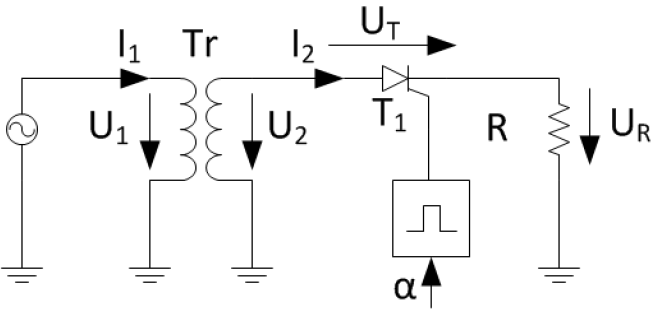
\includegraphics[width = \linewidth]{./pictures/m1c.png}}\\
  	\cline{1-2}
  Effektivwert 
  	&\ $U_{R RMS} = \sqrt{\frac{U_{2m}^2}{2\pi}\int\limits_{\alpha}^{\pi}sin^2(\beta) \cdot d\beta} = U_{2m} \cdot \sqrt{\frac{\pi-\alpha}{4\pi}+\frac{sin(2\alpha)}{8\pi}}$ &\\
  	\cline{1-2}
  Allgemein
  	&\ $\int\limits_{\alpha}^{\pi}sin^2(\beta) \cdot d\beta = \frac{\pi-\alpha}{2}+\frac{sin(2\alpha)}{4}$&\\
  	\cline{1-2}
\end{tabu}